
\documentclass[12pt,letterpaper]{article} 
\usepackage[letterpaper,left=3.5cm,right=3.5cm, top=3.0cm, bottom=3.0cm, footnotesep=1.0cm]{geometry} 
\usepackage{mathptmx}
\DeclareMathAlphabet{\mathcal}{OMS}{cmsy}{m}{n}
\usepackage[onehalfspacing]{setspace} 
\usepackage{fancyhdr} 
\usepackage{relsize}

\usepackage[bottom]{footmisc}
\usepackage{tabularx}
\usepackage{mathtools}
\pagestyle{empty}        


\usepackage{booktabs}    
\usepackage{natbib}      
\usepackage{bibentry}   

\usepackage{acronym}
\usepackage{multicol}

\usepackage{amsmath}
\usepackage{amssymb}
\usepackage{mathrsfs}
\usepackage{listings}
\usepackage{graphicx}
\usepackage{mathtools}
\usepackage[usenames,dvipsnames]{color}
\usepackage{hyperref}

\lstset{language=R,
  basicstyle=\small\ttfamily,
  stringstyle=\color{ForestGreen},
  otherkeywords={0,1,2,3,4,5,6,7,8,9},
  morekeywords={TRUE,FALSE},
  deletekeywords={data,frame,length,as,character},
  keywordstyle=\color{blue},
  commentstyle=\color{ForestGreen},
}


\begin{document}

\begin{center}\uppercase{Ludwig-Maximilians-University Munich}\end{center}
\begin{center}\uppercase{Department of Statistics}\end{center}

\vspace{3cm}

\title{Variable selection using grouped horseshoe priors}
\date{\vspace{-5ex}}
{\let\newpage\relax\maketitle}
\thispagestyle{empty}


\begin{center}
  \begin{large}
    \begin{Large}
      Bachelor's Thesis\\
    \end{Large}
    Department of Statistics  \\
  \end{large}
\end{center}
\begin{center}
  Author:\\
  \begin{large}
    Tobias Pielok\\
  \end{large}
\end{center}
\vspace{1cm}
\begin{center}
  \begin{large}
    Supervisor: Dr. Fabian Scheipl
  \end{large}
\end{center}

\begin{center}  \begin{large}
    Submission date: \\%\date{\today} \\
  \end{large}
\end{center}

\vspace{1,5cm}

\begin{center}
  \begin{large}
    \author{Tobias Pielok, B.Sc. (TUM)}\\
 \end{large}
  Marchgrabenplatz 5\\ 
  80805 Munich\\ 
  \url{t.pielok@campus.lmu.de}\\
  Matrikelnr.:  11381351\\
\end{center}


\newpage
\setcounter{page}{1}
\tableofcontents
\newpage


\pagestyle{fancy}
\fancyhf{}
\fancyhead[R]{\thepage}
\renewcommand{\headrulewidth}{0pt} 
\section*{Notation and Symbols}

\begin{tabular}{lll}
$\mathcal{B}_\mathcal{M}\bigotimes\mathcal{B}_\mathcal{N}$ & & product-$\sigma$-algebra generated by $\{M\times N :\; M\in\mathcal{B}_\mathcal{M}, N\in\mathcal{B}_\mathcal{N} \}$ \\
$\theta \in \mathbb{R}^d$ & & If $\theta$ is a random variable: $\theta$ maps to $\mathbb{R}^d$ \\
$\text{C}^+(0,a)$ & & standard half-Cauchy distribution on the positive reals with scale parameter a
\end{tabular}

\pagebreak
\section{Introduction}
% need of variable selection -> what is variable selection
% using horseshoe priors for grouped variables
% compressed results 
\pagebreak

\section{Basic Concepts}
The foundation of Bayesian horseshoe priors is based on the inference of the posterior distribution of the parameters, which can be attained by combining the prior knowledge of the parameters and the likelihood of the data, and will be introduced in section \ref{sec:BayInf}. In order of carrying out this inference it is necessary to sample from the posterior distribution.
In most cases this posterior distribution can be neither expressed in an analytical form nor are there standard samplers for it. Hence the HMC Method and its derivative NUTS will be shown in section \ref{sec:HMC}, with which it is possible to sample from the posterior distribution even in a high dimensional case. To express in this Bayesian framework the structure of grouped variables, on which the grouped horseshoe priors will be later used in section \ref{sec:hsg},  additive models will be introduced in section \ref{sec:AddMod}.
\subsection{Bayesian inference}
\label{sec:BayInf}
In Bayesian statistics the inference is carried out on the posterior distribution of a parameter $\tau$, after taking into account the realization of data $x$. In order of defining this posterior distribution thoroughly some rigorous definitions are needed:
Let $\mathcal{X}$ and $\mathcal{T}$ denote the \textit{sample space} and \textit{parameter space}, i.e. $\tau \in \mathcal{T}$ and $x \in \mathcal{X}$. Their $\sigma$-algebras will be called respectively $\mathcal{B}_\mathcal{X}$ and $\mathcal{B}_\mathcal{T}$. Also let the family of \textit{sampling distribution} $\mathcal{P} := \{P_\theta :\;\theta \in \mathcal{T}\}$, where $P_\theta$ is a probability measure over $(\mathcal{X}, \mathcal{B}_\mathcal{X})$. With these definitions a general \textit{statistical experiment} can be defined as $(\mathcal{X}, \mathcal{B}_\mathcal{X}, \mathcal{P})$ and for any given probability measure $\mu$ on $(\mathcal{T}, \mathcal{B}_\mathcal{T})$ a \textit{Bayesian experiment} can be identified with $(\mathcal{T}\times\mathcal{X},  \mathcal{B}_\mathcal{T}\bigotimes\mathcal{B}_\mathcal{X}, \Pi_{\mu,\mathcal{P}})$, where $\Pi_{\mu,\mathcal{P}}$ is the joint distribution of parameter-observation, s.t. $\forall T \in \mathcal{B}_\mathcal{T}, X \in \mathcal{B}_\mathcal{X}$:
\begin{equation}
\label{eq:likprio}
\Pi_{\mu,\mathcal{P}}(T,X) = \int_T P_\theta(X)\mu(d\theta ). 
\end{equation} 
The measure $\mu$ will be called the \textit{prior distribution} of the parameter. The \textit{predictive distribution} of the observations $P_{\mu,\mathcal{P}}$ is the marginal distribution of $\Pi_{\mu,\mathcal{P}}$ on $(\mathcal{X}, \mathcal{B}_\mathcal{X})$, s.t. $\forall X \in \mathcal{B}_\mathcal{X}: $
\begin{equation}
P_{\mu,\mathcal{P}}(X) = \Pi_{\mu,\mathcal{P}}(\mathcal{T},X).
\label{eq:pred}
\end{equation}
Eq. (\ref{eq:likprio}) can be rewritten with the predictive distribution (\ref{eq:pred}) and the family of \textit{posterior distributions} $\{\mu_\mathcal{P}(\cdot |\; x):\; x\in\mathcal{X}\}$, s.t. $\forall T \in \mathcal{B}_\mathcal{T}, X \in \mathcal{B}_\mathcal{X}$
\begin{equation}
\label{eq:post}
\Pi_{\mu,\mathcal{P}}(T,X) = \int_X \mu_\mathcal{P}(T|\; x) P_{\mu,\mathcal{P}}(dx ). 
\end{equation} 
Under the assumption that the Bayesian experiment $(\mathcal{T}\times\mathcal{X},  \mathcal{B}_\mathcal{T}\bigotimes\mathcal{B}_\mathcal{X}, \Pi_{\mu,\mathcal{P}})$ is dominated in the Bayesian setting (if not other stated, this will be assumed for the rest of the thesis) it can be shown (see [\cite{interbayes}]), that a posterior distribution for given $x$ can also be expressed with the Radon-Nikodym derivative, s.t. $\forall T \in \mathcal{B}_\mathcal{T}:$
\begin{equation}
\label{eq:dpost}
 \mu_\mathcal{P}(T|\; x) = \frac{\int_T \frac{dP_\theta}{d\lambda}(x)\mu(d\theta)}{\int_\mathcal{T} \frac{dP_\theta}{d\lambda}(x)\mu(d\theta)},
\end{equation} 
where $(\mathcal{X}, \mathcal{B}_\mathcal{X}, \mathcal{P}_C)$ is dominated by a finite measure $\lambda$. The function $\frac{dP_\theta}{d\lambda}$ is called \textit{likelihood function}. A class $\mathcal{P}_C$ of prior distributions is said to be a conjugate family for a class $\mathcal{F}$ of likelihood functions if  $\mu_\mathcal{P}(T|\; x) \in \mathcal{P}_C \; \forall T \in \mathcal{B}_\mathcal{T},  X \in \mathcal{B}_\mathcal{X}$.
%Why? -> inference%
\\An adequate choice of a point estimate to determine the location of the parameter $\theta$ depends on the underlying loss function. If a quadratic loss function $L$ is chosen, i.e. $L(\theta, \hat{\theta}) = ||\theta - \hat{\theta}||_2^2$, the expected loss $\mathbb{E}_{\theta \sim \mu} (L(\theta, \hat{\theta}))$ is minimized by the \textit{posterior mean} 
\begin{equation}
\label{eq:pmean}
	\hat{\theta} = E_{\theta |x \sim \mu_\mathcal{P}}(\theta |\; x),
\end{equation}
 if it exists (see [\cite{statdec}]). 
\\ A $100(1-\alpha)\%$ \textit{credible set} is a set $C \subset \mathcal{T}$, s.t.
\begin{equation}
1 - \alpha \leq P(C| \;x ) = \mu_\mathcal{P}(C|\; x).
\end{equation}
Which means that the parameter $\theta$ has the subjective probability of $(1-\alpha)$ that $\theta \in C$.
Because $C$ is not unique, additional constraints can be imposed on the solution. If the size of $C$, which can be defined as  $S(C) := \mu(C)$, is minimized one gets under mild conditions the  $100(1-\alpha)\%$  HDP credible set  as described in [\cite{statdec}], if there exists a posterior density $p_{\theta|\;x}$.
The  $100(1-\alpha)\%$ HDP credible set is defined as  
\begin{equation}
\label{eq:hdp}
C = \{\theta \in \mathcal{T}: \; p_{\theta|\;x}(\theta|\; x) \geq k(\alpha)\},
\end{equation}
where $k(\alpha)$ is the largest constant, s.t. $C$ is a $100(1-\alpha)\%$ credible set.
\newpage
\subsection{HMC and NUTS}
As already seen for carrying out the Bayesian inference the posterior distribution $\mu_\mathcal{P}$ is needed. In general solving Eq.  (\ref{eq:post}) or Eq. (\ref{eq:dpost}) for the posterior distribution is only in trivial cases analytically possible. Hence one tries to approximate the distribution by sampling from it. In most cases there is no standard sampler for $\mu_\mathcal{P}$. One way to overcome this problem, if there exist a corresponding probability density function $p(\theta)$ to $\mu_\mathcal{P}$, is to use the HMC method, where samples are drawn from a known distribution and with these samples of the desired distribution are computed. In HMC in order to sample a parameter $\theta$, for which it holds that $\theta \sim \mu_\mathcal{P}$ and $\theta \in \mathbb{R}^d$, an auxiliary variable $\rho$ is typically drawn from a multivariate normal distribution, s.t.
\begin{equation}
\rho \sim \mathcal{N}(0,\Sigma), 
\end{equation}
where $\rho \in \mathbb{R}^d$ and the covariance matrix $\Sigma \in \mathbb{R}^{d \times d}$. With the joint density $p(\rho, \theta)$ a so-called \textit{Hamiltonian} can be defined with regards of the canonical distribution as
\begin{equation}
H(\rho, \theta) = -\log p(\rho, \theta) = \underbrace{-\log p(\rho |\; \theta)}_{=:T(\rho |\; \theta)} \underbrace{-\log p(\theta)}_{=:V(\theta)},
\end{equation}
where T is called kinetic energy and V the potential energy. In general a Hamiltonian can be defined as follows:
Let $\rho,\theta \in (\mathbb{R}^d)^\mathbb{R}$ and $H(\rho,\theta)$ be scalar function sufficiently smooth.
$H$ is called a Hamiltonian if it holds that $\forall i \in \{1,\dots,d\}:$
\begin{equation}
\label{eq:hamdym}
\begin{aligned}
\frac{d \rho_i }{dt} = \frac{\partial H}{\partial \theta_i}, \\
\frac{d \theta_i }{dt} = -\frac{\partial H}{\partial \rho_i}.
\end{aligned}
\end{equation}
It can be shown that the Hamiltonian dynamics (\ref{eq:hamdym}) is reversible and preservers volume, which can even hold for the discretized version of the differential equations (see [\cite{mcmchb}]). With the \textit{leapfrog integrator}, which uses a discrete time step $\epsilon$, this can be achieved and (\ref{eq:hamdym}) can be solved numerically stable (see [\cite{mcmchb}]). Transitioning from a state $(\rho, \theta)$ to a new state $(\rho^*,\theta^*)$ in the leapfrog scheme, firstly a new  $\rho$ is drawn independently of $\theta$ and previous values of $\rho$ and secondly $L$ leapfrog steps are applied. One step of the leapfrog integrator can be summarized as follows:
\begin{enumerate}
\item The auxiliary variable $\rho$ is updated with half-step $\frac{\epsilon}{2}$ update using the negative derivative of the potential energy.
\label{en:f}
\item The parameter $\theta$ is updated with a full-step $\epsilon$ in the direction of the new $\rho$ multiplied with the derivative of the kinetic energy, which is represented by the covariance matrix $\Sigma$.
\item Another half-step $\frac{\epsilon}{2}$ update of $\rho$ as in \ref{en:f} is performed.
\end{enumerate}  
After $L$ leapfrog steps the proposal state $(\rho^*,\theta^*)$ is accepted as the new state with a probability of 
\[\min(1, \exp(H(\rho, \theta)-H(\rho^*,\theta^*))).
\] Otherwise $(\rho, \theta)$ is returned as the new state and hence also serves as the new initialization for the next iteration. This is called the Metropolis Accept Step.\\
 The series of by this scheme returned $\theta$ is also called a chain. As described in [\cite{convhmc}] under certain regularity conditions and control of the tail of posterior distribution $\mu_\mathcal{P}$ this chain is irreducible and (Harris) recurrent and $\mu_\mathcal{P}$ is its so-called invariant distribution. For a chain with these properties and under some additional assumptions it can be shown that with the use of ergodic theorems, that the chain  converges for almost every starting parameter $\theta_0$ in distribution to $\mu_\mathcal{P}$ and the law of large numbers and the central limit theorem are still valid, s.t. 
inferences (\ref{eq:pmean}) and (\ref{eq:hdp}) can be carried out approximately on a converged chain (see [\cite{mcstability}]). \\
The convergence speed of HMC is highly influenced by the hyper-parameters, i.e. the number of steps $L$, the step-size $\epsilon$ and the covariance matrix $\Sigma$.
One scheme to tune the parameter $L$ is NUTS. The advantage of using NUTS consists in its auto-tuning capability without the need to execute pre-runs. The general idea of NUTS can be described as follows: For the state $(\rho,\theta)$ the Hamiltonian dynamics are simulated randomly both forwards and backwards in time to guarantee time reversibility. In every step the steps taken in one direction are doubled. The algorithm is stopped for a current $(\tilde{\theta},\tilde{\rho})$ when 
\begin{equation*}
\frac{d}{dt}\frac{||\tilde{\theta} - \theta||^2_2}{2} = (\tilde{\theta} -\theta )^T\frac{d}{dt}(\tilde{\theta} - \theta) = (\tilde{\theta} -\theta )^T\Sigma\tilde{\rho} < 0,
\end{equation*} i.e. the expected squared jump distance would shrink and the dynamics could be described as an \textit{U-turn}. From these simulated states new proposals are sampled (for further details see [\cite{nuts}]). 
\label{sec:HMC}
\subsection{Bayesian approach to additive models}
Here the basic terminology related with additive models from a Bayesian perspective is recalled and the notation that will be used in the following is fixed. As a reference it is relied on [\cite{bayessm}]. \\
To study additive models firstly an understanding of univariate polynomial smoothing is helpful. For $n$ observation-pairs $(x_i, y_i)$, where $y$ is the output and $x$ is its covariate, with univariate polynomial smoothing a \textit{polynomial spline} $f(x)$ can be found, which fulfils 
\begin{equation}
y_i = f(x_i) + \epsilon_i,
\label{eq:polspline}
\end{equation}
where $\epsilon_i \sim \mathcal{N}(0,\sigma)$ for an Gaussian observation model. This polynomial spline $f$ of degree $D$ over $M+1$ (not necessarily equidistant) knots can be mathematically equivalent expressed in different spline bases, s.t.  
\begin{equation}
f(x) = \sum^K_{k=1}\gamma_k B_k(x),
\label{eq:pbasis}
\end{equation}
where $K = D + M.$
Commonly used spline bases are \textit{Truncated power series} and \textit{B-splines}. In this thesis the B-splines basis will be used, because of its superior numerical stability and its more adaptive Bayesian interpretation. Important to note is that B-splines form a local basis. With Eq. (\ref{eq:pbasis}) Eq. (\ref{eq:polspline}) can be written as a linear model for all observations, s.t.
\begin{equation}
\mathbf{y} = \mathbf{X} \mathbf{ \gamma } + \mathbf{\epsilon},
\end{equation}
where $\mathbf{X}$ contains the basis function evaluated at the observed covariate $\mathbf{x}$. \\
With higher node (and polynomial) degree polynomial splines are more prone to overfitting. To counter this \textit{P-splines} are used. Because for B-splines $\mathbf{\gamma}$ represents local regression coefficients, high differences of neighbouring $\gamma_i$ should be penalized. Hence the so-called \textit{penalized least-squares} (PLS) criterion can be formulated for B-splines with equidistant knots as
\begin{equation}
PLS(\lambda) = ||\mathbf{y} - \mathbf{X}\mathbf{\gamma}||^2_2 +
 \lambda||\mathbf{D}_d\mathbf{\gamma}||^2_2 = ||\mathbf{y} - \mathbf{X}\mathbf{\gamma}||^2_2 +  \lambda\mathbf{\gamma}^T\underbrace{\mathbf{D}_d^T\mathbf{D}_d}_{=:\mathbf{K}}\mathbf{\gamma},
\end{equation}
where $\mathbf{D}_d \in \mathbb{R}^{(\mathbf{K}-d) \times \mathbf{K}}$ is the so-called \textit{difference matrix} of order $d$ and $\mathbf{K}$ the penalty matrix. The PLS criterion can be equivalently defined by using a $d^{\text{th}}$ random walk prior distribution for $\mathbf{\gamma}$, s.t. 
\begin{align}
\begin{split}
p(\mathbf{\gamma}, \sigma^2 | \; \mathbf{y}) & \propto  p(\mathbf{y} | \; \mathbf{\gamma}, \sigma^2) p(\mathbf{\gamma} | \; \tau^2) p(\sigma^2) p(\tau^2) \\
& \propto  \exp(-\frac{1}{2\sigma^2}||\mathbf{y} - \mathbf{X}\mathbf{\gamma}||^2_2)
(\frac{1}{\tau^2})^{\text{rank}(\mathbf{K})/2}\exp(-\frac{1}{2\tau^2}\mathbf{\gamma}^T\mathbf{K}\mathbf{\gamma}) \cdot \\
 &  \quad\cdot p(\sigma^2) p(\tau^2),
\end{split}
\end{align}
where typically prior distributions of $\sigma^2$ and $\tau^2$ are chosen, s.t. 
\begin{equation}
\sigma^2 \sim \text{IG}(a_\sigma, b_\sigma), \tau^2 \sim \text{IG}(a, b).
\end{equation}
Note because $\mathbf{K}$ has no full rank, which can be clearly seen from its construction, this means that for $\mathbf{\gamma}$ a degenerate Gaussian distribution is assumed. \\
Now considering the case of multiple covariates $\mathbf{x}_1, \dots , \mathbf{x}_p$ for an output $\mathbf{y} \in \mathbb{R}^n$ it is possible to extend the smoothing splines analogously to this multivariate setting, but by doing this the number of parameter rises quickly and so does the amount of data, which would be needed to identify these. Hence one commonly used technique is to restrict the model to an additive structure, s.t. the so-called additive model\footnote{In this thesis only additive model containing one dimensional splines will be used, but in general additive model can be also composed from higher dimensional smoothing functions.} for $\mathbf{y}$ can be written as
\begin{equation}
\mathbf{y} = \mathbf{U}\mathbf{\beta} +  \sum^{m_s}_{i=1} \mathbf{f}_i(\mathbf{x}_i) + \mathbf{\epsilon},
\label{eq:am}
\end{equation}
where $\mathbf{\epsilon} \sim \mathcal{N}(0, \sigma^2)$ and $\mathbf{U}\in \mathbb{R}^{n\times m_{p}} $ denotes the model matrix of predictors $\mathbf{u}_1,\dots\mathbf{u}_{m_l}$, which are modelled linearly, with associated parameter vector $\mathbf{\beta} \in \mathbb{R}^{ m_{p}}$ and $\mathbf{f}_i$ the vector of one dimensional smoothing function to the corresponding covariate $\mathbf{x}_i$, which is defined $\forall i \in \{1,\dots ,m_{s}\}$. Every $\mathbf{f}_i$ can expressed as 
\begin{equation}
\mathbf{f}_i(\mathbf{x}_i) = (f_i(x_{i1}),\dots,f_i(x_{in}))^T = (\sum^{K_i}_{k=1}\gamma_{ik} B^i_k(x_{i1}),\dots,\sum^{K_i}_{k=1}\gamma_{ik} B^i_k(x_{in}))^T.
\label{eq:mvsf}
\end{equation}
To ensure the identifiability of the single $\mathbf{f}_i$ an artificial centering constraint is introduced, s.t. $\forall i \in \{1,\dots ,m_{s}\}$ it holds that
\begin{equation}
\sum^n_{j=1}f_i(x_{ij}) = 0.
\end{equation}  
The linearity of Eq. (\ref{eq:mvsf}) can be expressed, s.t. 
\begin{equation}
\mathbf{f}_i(\mathbf{x}_i) = \mathbf{X}_i\mathbf{\gamma}_i.
\label{eq:matmvsf}
\end{equation}
With Eq. (\ref{eq:matmvsf}) the additive model (\ref{eq:am}) can be written as
\begin{equation}
\mathbf{y} = \mathbf{U}\mathbf{\beta} +  \sum^{m_s}_{i=1} \mathbf{X}_i\mathbf{\gamma}_i + \mathbf{\epsilon}.
\label{eq:matam}
\end{equation}
To estimate the regression coefficients of the additive model (\ref{eq:matam}) without overfitting the extended PLS criterion, which is to be minimized, based on the estimated output $\eta = \mathbf{U}\mathbf{\beta} +  \sum^{m_s}_{i=1} \mathbf{X}_i\mathbf{\gamma}_i$
can be used, which can be formulated as
\begin{equation}
\text{PLS}(\gamma_1,\dots ,\gamma_{m_s},\mathbf{\beta}) = (\mathbf{y} - \mathbf{\eta})^T(\mathbf{y} - \mathbf{\eta}) + \sum^{m_s}_{i=1} \mathbf{\lambda}_i\mathbf{\gamma}_i^T\mathbf{K}_i\mathbf{\gamma}_i,
\end{equation}
where $\mathbf{K}_i$ is the penalty matrix of $\mathbf{f}_i$. In the Bayesian framework the extended PLS criterion can be modelled, s.t. it holds for the posterior distribution of the regression coefficients that 
\begin{align}
\begin{split}
p(\gamma_1,\dots ,\gamma_{m_s},\mathbf{\beta},\tau^2_1,\dots,\tau^2_{m_s},\sigma^2| \; \mathbf{y}) \propto &
(\frac{1}{\sigma^2})^{n/2}\exp(-\frac{1}{2\sigma^2}(\mathbf{y} - \mathbf{\eta})^T(\mathbf{y} - \mathbf{\eta})) \cdot \\
& \cdot p(\mathbf{\beta}) \cdot \prod^{m_s}_{i=1}(\frac{1}{\tau^2_i})^{\text{rank}(K)/2}\exp(\frac{1}{2\tau_i^2}\mathbf{\gamma}_i^T\mathbf{K}_i\mathbf{\gamma}_i) \cdot \\
& \prod^{m_s}_{i=1}  p(\tau^2_i)  \cdot  p(\sigma^2),
\end{split}
\end{align}
i.e. the posterior mean is consistent with the PLS criterion. Typically a weakly informative prior distribution is used for $\mathbf{\beta}$, s.t. $\mathbf{\beta} \sim N(\mathbf{c},\mathbf{C})$, where $\mathbf{C}$ is a 'large' covariance matrix. Because in this setting the sample density of $\mathbf{y}$ is normal and by using the fact that the normal distribution is a conjugate family for these, it can be easily shown that the full conditionals $\mathbf{\beta} |\; \cdot \sim N(\mu_\beta, \Sigma_\beta)$ with
\begin{align}
\Sigma_\beta = \sigma^2(\mathbf{U}^T\mathbf{U} + \sigma^2 \mathbf{C}^{-1})^{-1}, \\
\mu_\beta = \frac{1}{\sigma^2}\Sigma_\beta(U^T(\mathbf{y} - \eta + \mathbf{U}\mathbf{\beta}) + \sigma^2\mathbf{C}^{-1}\mathbf{c}).
\label{eq:mubeta}
\end{align}


\label{sec:AddMod}
\pagebreak

\section{Bayesian horseshoe}
When applying the Bayesian horseshoe technique for variable selection so-called horseshoe prior distribution is assumed for the parameters of interest, which main idea consist in using a global shrinkage parameter while allowing for an \textit{informative} parameter to escape the shrinkage trough a local shrinkage parameter. The mathematical foundations of this type of prior distribution is described in section \ref{sec:mfound}. In section \ref{sec:hsg} these ideas will be extended to the case of grouped variables. In situations where the parameters can not be identified well through the data, the hyperprior choice of the global shrinkage parameter can influence the results strongly. Because of this a possible hyper prior choice is introduced in section \ref{sec:opt}. The implementation of the horseshoe priors, which will be applied on simulated data in section \ref{sec:sim}, uses ideas from section \ref{sec:pract}.
\subsection{Mathematical foundations}
\label{sec:mfound}
In [\cite{Carvalho2010}] the horseshoe prior is introduced as an estimation model for an observed $p$-dimensional vector $\mathbf{b}|\; \beta \sim N(\beta, \sigma^2I)$, where $\beta$ is assumed to be sparse.
In this model it is assumed $\forall i \in \{1,\dots,p\}$ that
\begin{equation}
\beta_i |\; \lambda_i \sim N(0,\lambda^2_i),\quad \lambda_i |\; \tau \sim \text{C}^+(0, \tau), \quad \tau \sim  \text{C}^+(0, \sigma).
\label{eq:hs}
\end{equation}
To understand the properties of this model better a linear Gaussian regression model is assumed for section \ref{sec:mfound}, s.t. for an observed output $\mathbf{y}$ it holds that 
\begin{equation}
\mathbf{y} = U\beta + \epsilon.
\label{eq:gaus}
\end{equation}
In the case of (\ref{eq:gaus}) if follows from (\ref{eq:hs}) that the prior distribution of $\beta$ is s.t. $\beta \sim N(0, \tau^2\Delta), $ where $\Delta$ is a diagonal matrix with $\lambda_i^2$ as its diagonal entries. By plugging these values into (\ref{eq:mubeta}) one gets that the posterior expected mean of $\beta$
\begin{equation}
\mu_\beta = (\mathbf{U}^T\mathbf{U} + \sigma^2 \frac{1}{\tau^2}\Delta^{-1})^{-1}\mathbf{U}^T\mathbf{y}.
\label{eq:mubetagaus}
\end{equation}
Since $\Delta$ is a diagonal matrix (\ref{eq:mubetagaus}) can be rewritten as 
\begin{equation}
\mu_\beta = \tau^2\Delta(\sigma^2(\mathbf{U}^T\mathbf{U} )^{-1} + \tau^2\Delta)^{-1}\underbrace{(\mathbf{U}^T\mathbf{U} )^{-1}\mathbf{U}^T\mathbf{y}}_{=:\hat{\beta}},
\label{eq:mubetagausmax}
\end{equation}
where $\hat{\beta}$ denotes the maximum likelihood solution. In the case of zero mean and uncorrelated predictors with unit variance it holds that $\mathbf{U}^T\mathbf{U} \approx nI$, s.t. (\ref{eq:mubetagausmax}) can be component-wisely approximated as 
\begin{equation}
\mu_{\beta_j} = (1-\kappa_j)\hat{\beta}_j,
\end{equation}
where 
\begin{equation}
\kappa_j = \frac{1}{1+n\sigma^{-2}\tau^2\lambda^2_j}
\end{equation}
is the so-called shrinkage factor for the j'th component of $\beta$. This name makes sense, since $n\sigma^{-2}\tau^2\lambda^2_j > 0$ it follows that $\kappa_j \in (0,1)$ and hence the limiting case of $\kappa = 1$ represents full shrinkage, where $\mu_{\beta_j} = 0$, and the other limiting case of $\kappa = 0$ no shrinkage, where $\mu_{\beta_j} = \hat{\beta}_j$.
By using (\ref{eq:hs}) and applying the transformation theorem it can be shown, that the conditional density of $\kappa_j$
\begin{equation}
p(\kappa_j|\;\tau,\sigma) = \frac{1}{\pi}\frac{\sigma^{-1}\tau\sqrt{n}}{(n\sigma^{-2}\tau^2 - 1)\kappa_j + 1}\frac{1}{\sqrt{\kappa_j}\sqrt{1-\kappa_j}}. 
\label{eq:kappa}
\end{equation}
\begin{figure}[bt!]
 \centering
 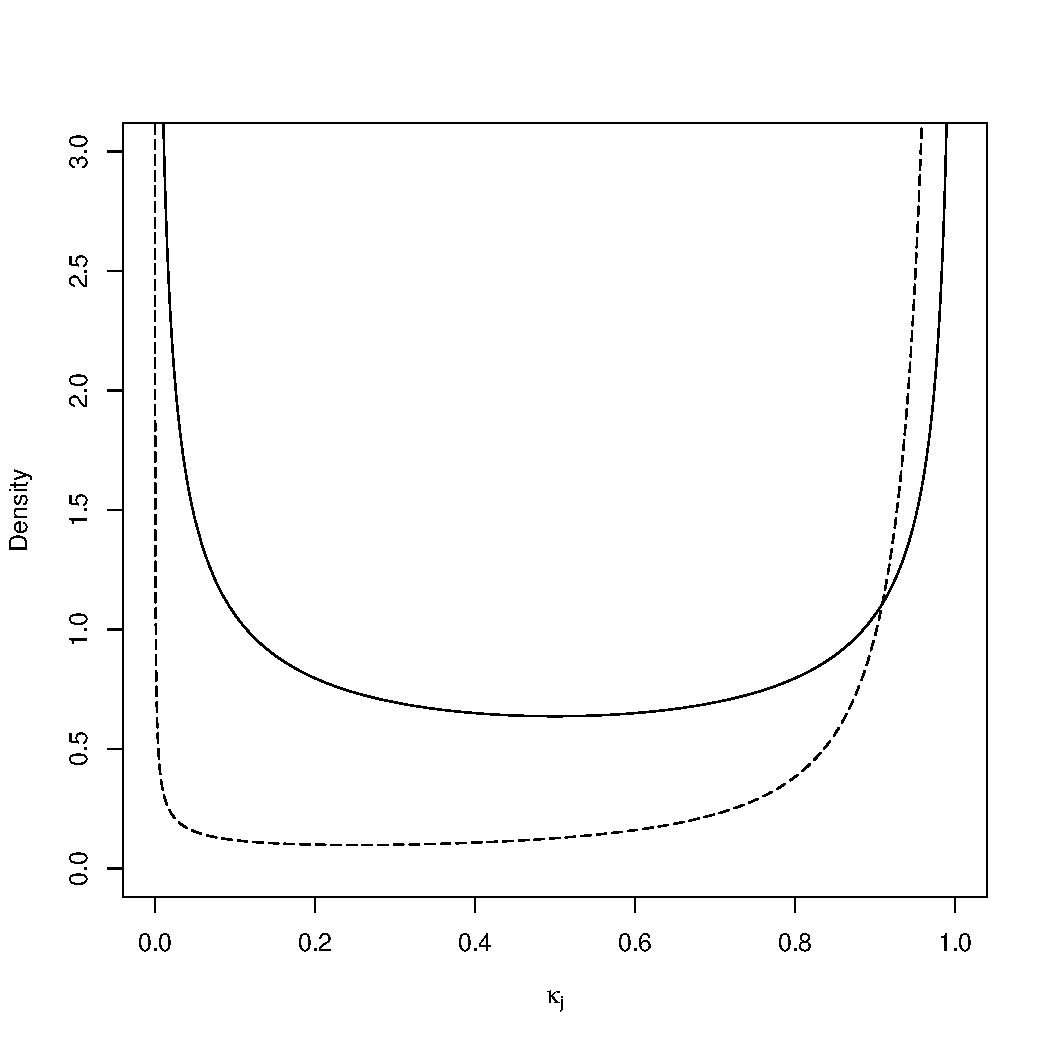
\includegraphics[width=0.5\textwidth]{../plots/kappa.pdf}
 \caption{Conditional density of the shrinkage factor $\kappa_j$ for $n\sigma^{-2}\tau^2 = 1$ (solid) and 
 for $n\sigma^{-2}\tau^2 = 0.1$ (dashed).}
 \label{fig:hs}
\end{figure}
For $n\sigma^{-2}\tau^2 = 1$ it holds that $\kappa_j \sim \text{Beta}(\frac{1}{2},\frac{1}{2})$ and its horseshoe resembling density can be seen in Fig. \ref{fig:hs}, from which the name of this method was derived. While under $n\sigma^{-2}\tau^2 = 1$ equal probability mass is distributed on shrinkage and no shrinkage, under  $n\sigma^{-2}\tau^2 = 0.1$ more mass is distributed towards $1$, which means that shrinkage is favoured.


\subsection{Extending horseshoe prior to the case of grouped variables}
\label{sec:hsg}
In additive models two natural group structures arise:
\begin{enumerate}
\item A categorical predictor with $m_{G_1}$ levels can be modelled with $m_{G_1} -1$ dummy coded variables, which represent a group of $m_{G_1} - 1$ linear predictors.
\item A smoothing function with parameter $\mathbf{\gamma} \in \mathbb{R}^{K_1}$ also can be seen as a group of $K_1$ parameters. 
\end{enumerate}
Because one usually wants a smooth function defined on the whole domain and does not want to select categorical predictors level-wise, the horseshoe prior can be straightforwardly extended for this grouped structures, s.t. for an additive model as defined in (\ref{eq:am}), where the $g$ linear predictors are categorical with number of levels $m_{G_i}$ and where the parameter vector $\gamma_j \in \mathbb{R}^{K_j}$ of the $m_s$ smoothing functions,
\begin{align}
\beta|\; \sigma^2,\tau^2, \lambda^2_{11},\dots,\lambda^2_{1g} \sim N(0, \sigma^2\tau^2\mathbf{D}_{\lambda_1}),\\
\forall j \in  \{1,\dots,m_s\}\quad \gamma_j  \sim N(0, \tau^2\lambda_{2j}^2\mathbf{K}_j),
\end{align}
where $\mathbf{D}_{\lambda_1} = \text{diag}(\lambda_{11}^2I_{m_{G_1}},\dots,\lambda_{1g}^2I_{m_{G_g}})$ and 
\begin{align*}
\lambda_{1i}|\;\tau \sim C^+(0,\tau), \quad \lambda_{2i}|\;\tau \sim C^+(0,\tau), \quad \tau^ \sim C^+(0,1).
\end{align*}
This means every group structure has one local shrinkage parameter. Hence the whole group is either shrunken as a whole or stays not shrunken.
\subsection{Hyperprior choice for global shrinkage parameter}
\label{sec:opt}
In [\cite{horseshoe}] it is shown that for the global shrinkage parameter the choice of scale 1 can produce suboptimal results  in settings where $\tau$ can not well be identified by the data, e.g high ratio of number of parameter to number of data or very noisy data. Hence the authors propose to introduce $\tau_0$ as an hyper-parameter, s.t. $\tau \sim C^+(0,\tau_0)$ and show that an good way to choose this parameter is by using an guess of the number of relevant variables $p_0$ of of all the $D$ to be shrunken variables, s.t.
\begin{equation}
\tau_0 = \frac{p_0}{D-p_0}\frac{\sigma}{\sqrt{n}}.
\label{eq:tau0}
\end{equation}
In this thesis it will be shown, that this choice of $\tau_0$ is still reasonable in the setting of grouped variables as discussed in section \ref{sec:hsg}: \\
Now consider the grouped variables setting of section \ref{sec:hsg}. 
Every group has its own local shrinkage coefficient $\kappa_{ij}$.
From the prior distribution of $\kappa_{ij}$ (\ref{eq:kappa}) it follows that
\begin{equation}
\mathbb{E}(\kappa_{ij}|\; \tau, \sigma) = \underbrace{\frac{1}{1+\sigma^{-1}\tau\sqrt{n}}}_{=:\mu_\kappa}.
\end{equation}
Since $\kappa_{ij}$ is typically is either near zero or near one it motivates the definition of effective number of parameter $m_{\text{eff}}$ as 
\begin{equation}
m_{\text{eff}} = \sum^g_{i=1}(1-\kappa_{1i})m_{G_i} + \sum^{m_s}_{j=1}(1-\kappa_{2j})K_j.
\label{eq:meff}
\end{equation}
By taking the expectation of (\ref{eq:meff}) it follows that
\begin{equation}
\mathbb{E}(m_{\text{eff}}|\; \tau, \sigma) = (1-\mu_\kappa)\underbrace{( \sum^g_{i=1}m_{G_i} + \sum^{m_s}_{j=1}K_j)}_{=: D} = \frac{\sigma^{-1}\tau\sqrt{n}}{1+\sigma^{-1}\tau\sqrt{n}}D.
\label{eq:meffg}
\end{equation}
By solving (\ref{eq:meffg}) for $\tau$ for an guess of the effective number of parameter $p_0$ the same proposal as presented in (\ref{eq:tau0}) is derived. The integration of $\tau_0$ in the model can be done in other ways than using $\tau \sim C^+(0,\tau_0)$, e.g. fixing $\tau$ to $\tau_0$ or using $\tau \sim N^+(0,\tau_0)$. The effects of these other approaches are discussed in [\cite{horseshoe}].
\subsection{Practical aspects}
\label{sec:pract}

\pagebreak

\section{Simulations}
\label{sec:sim}
\subsection{Settings}

\subsection{Szenario 1}
\subsubsection{Data generation}
\subsubsection{Results}
\subsection{Szenario 2}
\subsubsection{Data generation}
\subsubsection{Results}

\subsection{Summary}
\pagebreak

%\section{Benchmarking}

%\subsection{Regression}
%\subsubsection{Data description}
%\subsubsection{Comparisions and Results}
%\subsection{Classification}
%\subsubsection{Data description}
%\subsubsection{Comparisions and Results} 

\subsection{Summary}

\pagebreak

\section{Conclusions}
\pagebreak
\section{Appendix}
\subsection{Other variable selection methods}
\subsubsection{Spike-and-slab variable selection}
\subsubsection{Feature selection using LASSO}
\pagebreak
\subsection{Code}
\pagebreak

\pagestyle{fancy}
\bibliographystyle{apalike}
\bibliography{thesis} 

\nocite{*} 
\addcontentsline{toc}{section}{Bibliography}
\clearpage

\listoffigures
\addcontentsline{toc}{section}{List of Figures}
\clearpage


\section*{List of Abbreviations}
\addcontentsline{toc}{section}{List of Abbreviations}
\begin{multicols}{2}
  \begin{acronym}[abr]
    \acro{HMC}{Hamiltonian Monte Carlo}
    \acro{NUTS}{No-U-Turn Sampler}    
    \acro{HDP}{highest posterior density}       
    \acro{MCMC}{Markov Chain Monte Carlo}
    \acro{PLS}{penalized least-squares}
  \end{acronym}
\end{multicols}



\pagebreak
\subsection*{Statement}
\label{erklaerung}
\vspace*{0.5cm}
I hereby declare that this thesis is my own original work and that all sources have been acknowledged.\\[1.0cm]
Munich, \today \\[2.0cm]
\rule{6.0cm}{0.4pt} \\
Tobias Pielok


\end{document}
